\chapter{\leavevmode\newline The Standard Model of Particle Physics}
\label{chap:chapter_1}
Several particles were discovered after years of experimental observations, and this led to the development of the Standard Model (SM) during the 1970s. The SM is a Quantum Field Theory (QFT) based on the symmetries of the Lie group, SU(3)$ \times$ SU(2)$ \times$ U(1) \cite{stiller2016full}. It not only describes the fundamental particles and interactions (except for gravitation) but also predicts new particles. The fundamental particles in the SM have a property known as spin and are divided into two main groups: fermions and bosons, as shown in Fig \ref{fig:sm}.

Fermions obey the Pauli exclusion principle, have $\frac{1}{2}$-spin, and there exists an antiparticle with the same properties but opposite quantum numbers, such as electric charge. They are subdivided into quarks and leptons, with both groups having six particles, and they are further grouped into three generations according to their mass. Quarks are always found in bound states known as hadrons, a meson is formed by bounded state of a quark and an antiquark, and a baryon is formed by three bounded quarks \cite{stiller2016full, fedi2016studies, grummer2021search}. Quarks have an electrical charge of $+\frac{2}{3}e$ (u, c, t) or $-\frac{1}{3}e$ (d, s, b), as well as a color charge, and can thus interact with the strong force. On the other hand, leptons have an electrical charge of $-1e$ (e, $\mu$, $\tau$) or are neutral (the corresponding neutrinos, $\nu_e, \nu_\mu, \nu_\tau$) and they don't interact with the strong force \cite{bonanomi2021response, bragagnolo2021measurement}.

Bosons have integer spin and are known as force or interaction carriers and are divided into vector and scalar bosons. The scalar boson is the Higgs boson, and it gives the other elementary particles mass. The vector bosons are related to the fundamental interactions. The photon $\gamma$ is a massless and neutral particle that mediates the electromagnetic interaction between electrically charged particles. The massive bosons, $W^{\pm}$ and $Z$, mediate the weak force between fermions. Finally, gluons mediate the strong interaction between quarks \cite{grummer2021search, bragagnolo2021measurement}.

SM is considered the most successful theory developed by mankind. However, it does not explain a number of physical phenomena. For instance, the existence of three and only three generations of fermions. It does not account for gravity, and to date, there has been no observation of the vector boson responsible for the gravitational interaction, also known as the graviton. It also does not explain why there is more matter than antimatter in the universe, among other properties \cite{grummer2021search, danilov2020measurement}.
\begin{figure}[htp!]
	\centering
	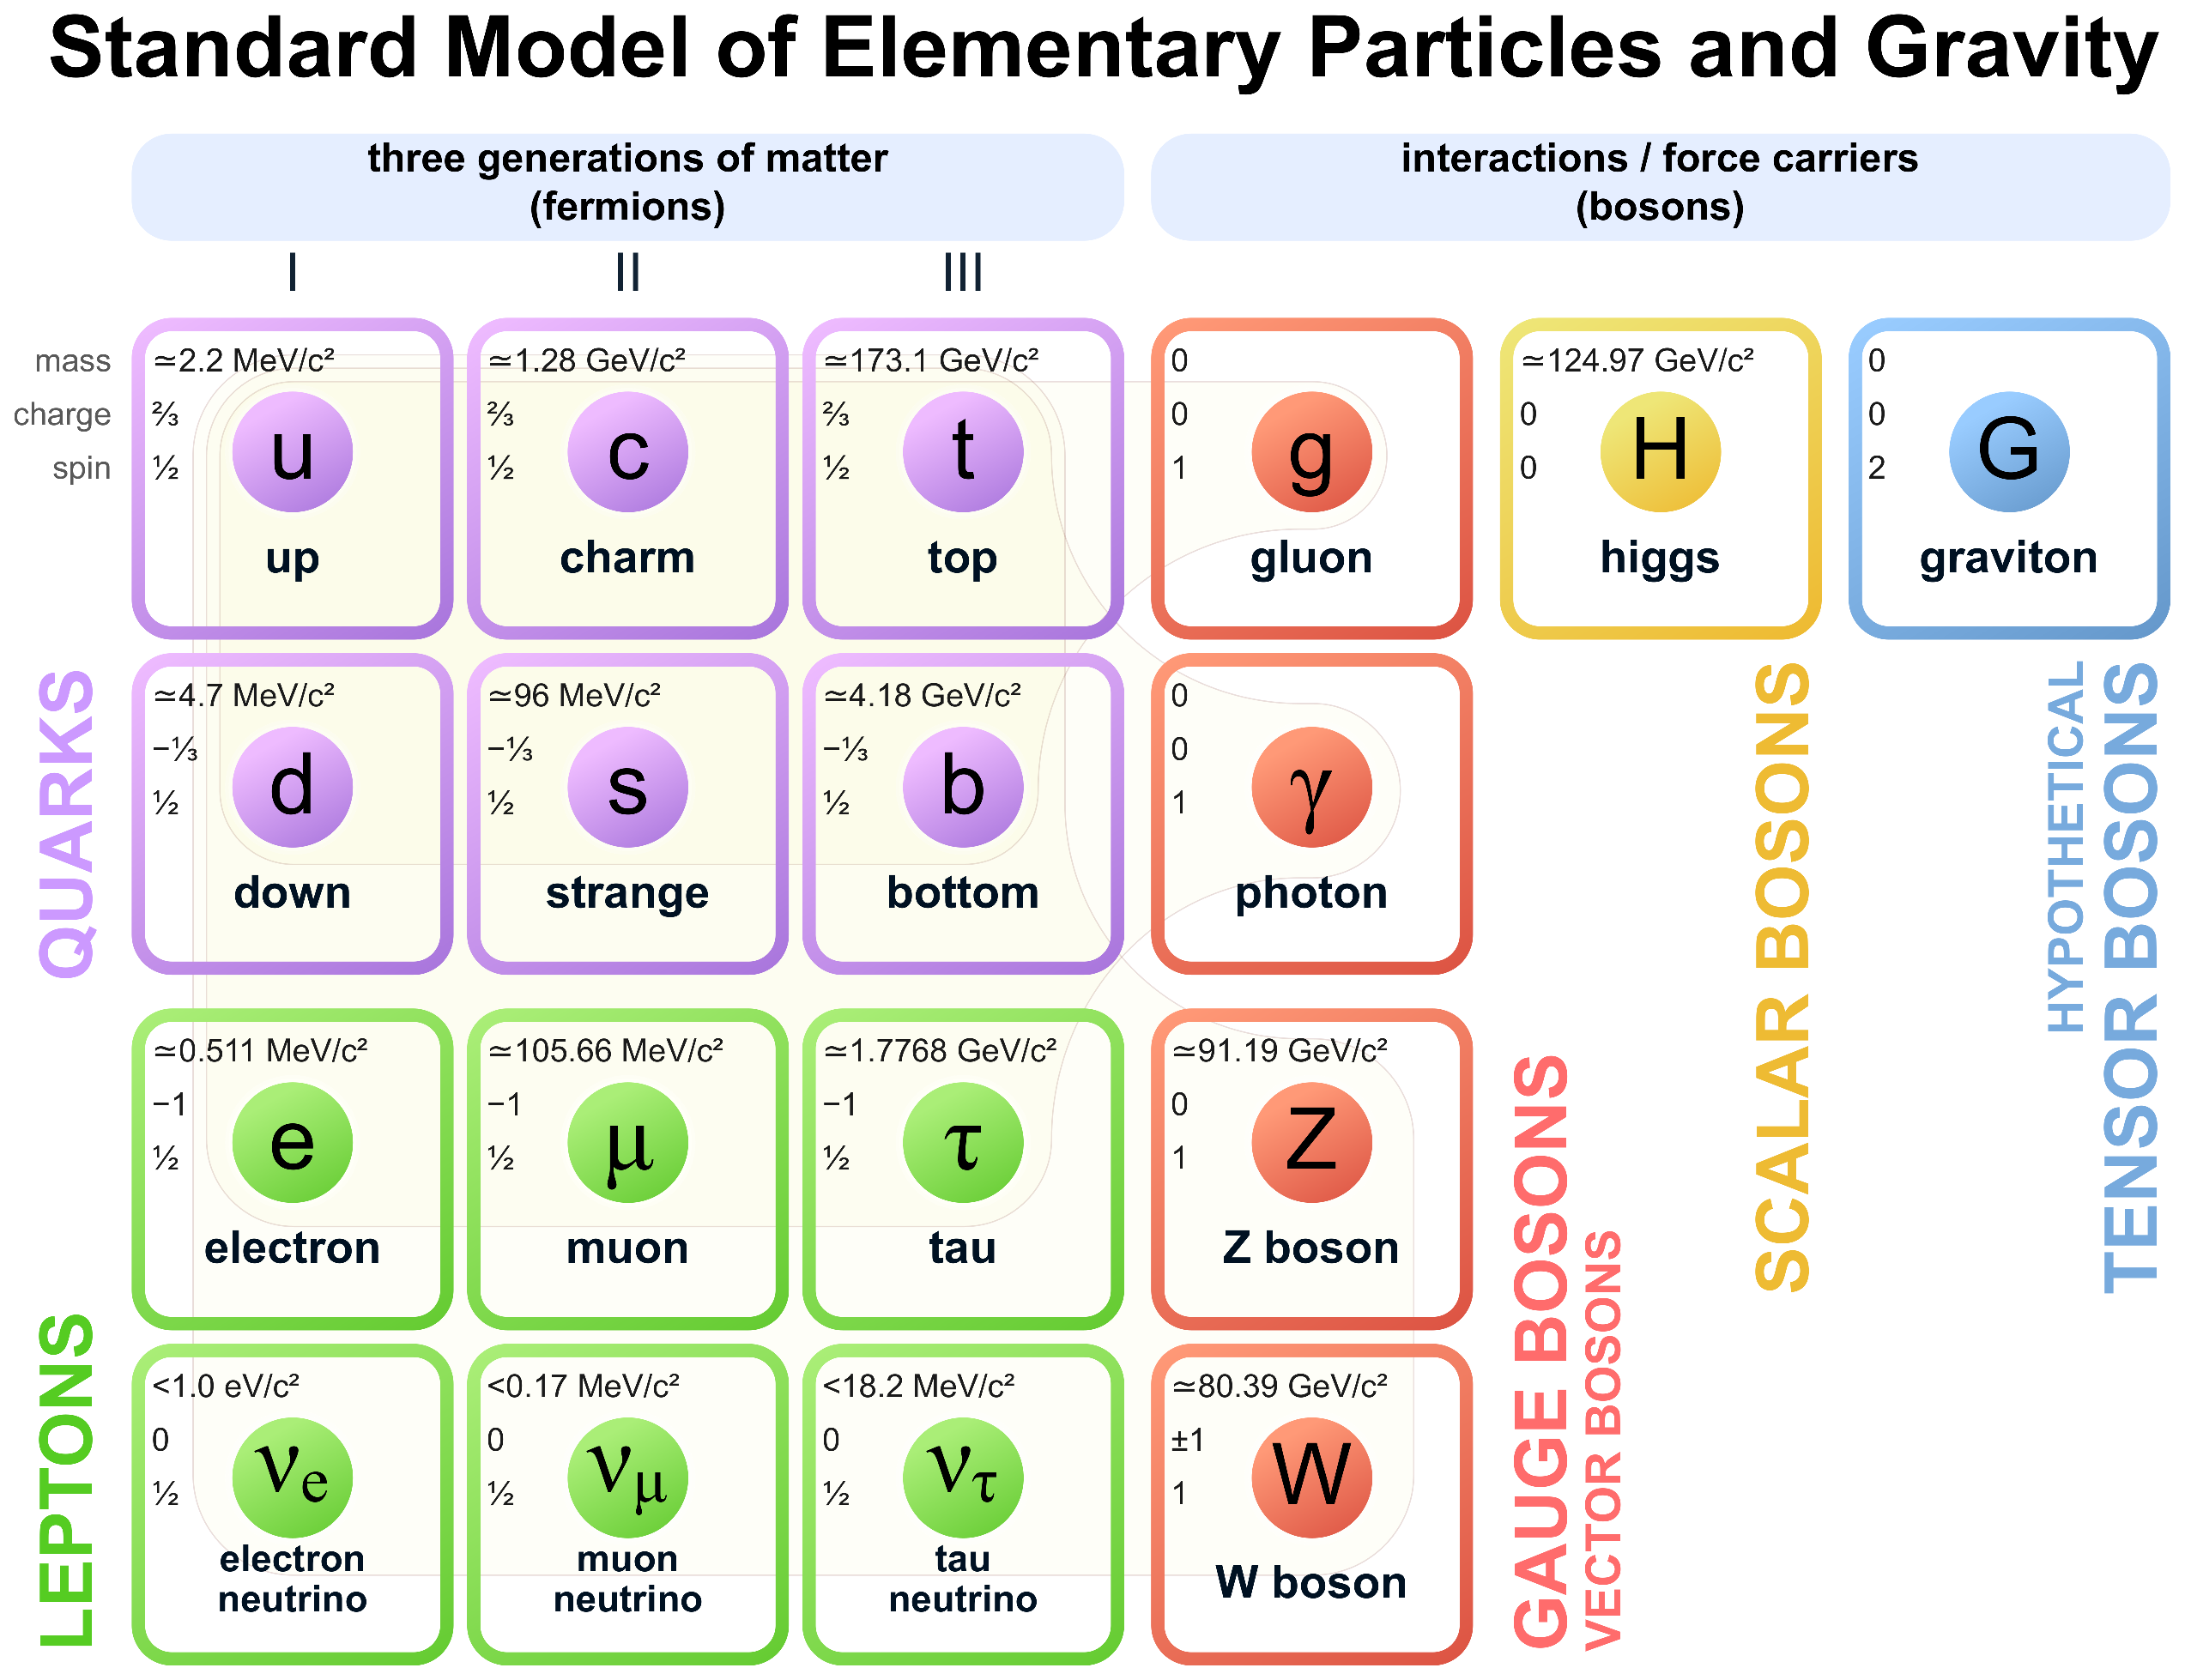
\includegraphics[scale=0.34]{MainContent/Figs/SM.eps}
	\caption{The Standard Model of fundamental particles. Retrieved from \cite{danilov2020measurement}.}
	\label{fig:sm}
\end{figure}

\section{QCD}
The theory in the SM that describes the strong interactions between colored quarks and gluons is known as Quantum Chromodynamics (QCD). QCD is symmetric under the group SU(3)$_C$, where C stands for color, and similar to the conservation of electrical charge in Quantum Electrodynamics (QED), there is a conserved property known as the color charge with a corresponding anti-color charge. Color charge exists in quarks. This charge comes in three flavors: red (r), blue (b), and green (g). Eight massless gluons mediate the strong interaction and have color charge, allowing them to interact with one another via the strong force.

To date, colored quarks have not been observed in free states, but rather in colorless bounded states known as hadrons. This is referred as "color confinement", and it is thought to be a direct result of gluons having a color charge. The observed hadronic states include mesons (one quark and one antiquark), baryions (three quarks), and pentaquarks (four quarks and one antiquark), which were confirmed in 2015 by the LHCb experiment. The hadronisation process is also a consequence of color confinement.  In this process, a cascade of mesons and baryons known as jets are produced when quarks and gluons group together interactively during gluon-gluon, quark-quark, or quark-gluon collisions.  The HCAL, which is described in the section \ref{cal_sys}, detects jets.

Asymptotic freedom is another interesting property of QCD. When the distance between quarks decreases, their transfer of momentum increases, but their coupling constant decreases as well. As a result, they do not interact as strongly with one another. Therefore, in this asymptotic limit, quarks and gluons can be approximated as free particles, in contrast to what happens in color confinement. It is also worth mentioning 

\section{$B^0_s$}
\subsection{$B^0_s \to J/\psi\phi$}
